\section{Results}

The extensive experimentation, summarized in Table \ref{tab:autoencoder_configs}, allowed for a deep analysis of the different architectural configurations. In this section, we present the quantitative, qualitative, and comparative results of the most relevant models.

\subsection{Performance on Synthetic Data}

The models were initially evaluated based on their Mean Squared Error (MSE) on a synthetic test set of 1000 images, kept separate from the training data. Table \ref{tab:mse_results} summarizes the performance of the top-performing architectures and other relevant cases.

The results clearly indicate that deeper architectures with three convolutional layers (A13, A15, A16) achieved the best performance, with MSE values around $0.0023$. This suggests that a hierarchical feature extraction is crucial for effectively modeling and removing speckle noise. Notably, the dimensionality of the latent space in these top models ($128$ or $256$) also played a significant role.

Furthermore, we observed that training duration did not linearly correlate with better performance. For instance, model A16, trained for only 70 epochs, achieved a performance nearly identical to A15 (trained for 500 epochs), suggesting that well-designed architectures can converge rapidly. This is a key finding, as it points towards more efficient training strategies. Several models, particularly shallower ones with long training times (e.g., A4), exhibited signs of overfitting, with a test MSE more than 25\% higher than their final training MSE.

\begin{table}[htbp]
\centering
\caption{Test MSE results for a selection of autoencoder configurations, ordered by performance. The table highlights the best models, an underperforming one, and a case with significant overfitting.}
\label{tab:mse_results}
\scriptsize
\begin{tabular}{|c|c|c|c|c|}
\hline
\textbf{Rank} & \textbf{Config.} & \textbf{Architecture Details} & \textbf{Test MSE} & \textbf{Comment} \\
\hline
1 & A15 & 3 Conv, 256 Dim, 500 Epochs & 0.002319 & Best performance \\
2 & A13 & 3 Conv, 128 Dim, 500 Epochs & 0.002346 & Excellent performance \\
3 & A16 & 3 Conv, 256 Dim, 70 Epochs  & 0.002348 & Best short-training model \\
4 & A7  & 2 Conv, 128 Dim, 500 Epochs & 0.002433 & Best 2-layer model \\
... & ... & ... & ... & ... \\
16 & A4 & 1 Conv, 32 Dim, 500 Epochs  & 0.002781 & High overfitting (+28.5\%) \\
... & ... & ... & ... & ... \\
23 & A1 & 1 Conv+Pool, 32 Dim, 5 Epochs & 0.005695 & Underperforming base model \\
\hline
\end{tabular}
\end{table}

\subsection{Visual Assessment and Architectural Insights}

Quantitative metrics are essential, but a visual assessment is crucial to understand the filter's behavior. Figure \ref{fig:imtest_A15} shows the result of applying the best-performing model, A15, to a sample synthetic test image.

The autoencoder demonstrates a remarkable ability to reduce speckle and reconstruct the mean gray levels of the homogeneous areas. However, the filtered image is not a perfect replica of the clean target. The model tends to introduce smooth, spatially correlated patterns, a common artifact of convolutional networks that are trained to find structure in images. This shows a fundamental challenge: the network struggles to distinguish between the speckle noise to be removed and the random texture inherent to the backscatter signal, which should be preserved. This behavior was consistent across all high-performing architectures.

\begin{figure}[htbp]
    \centering
    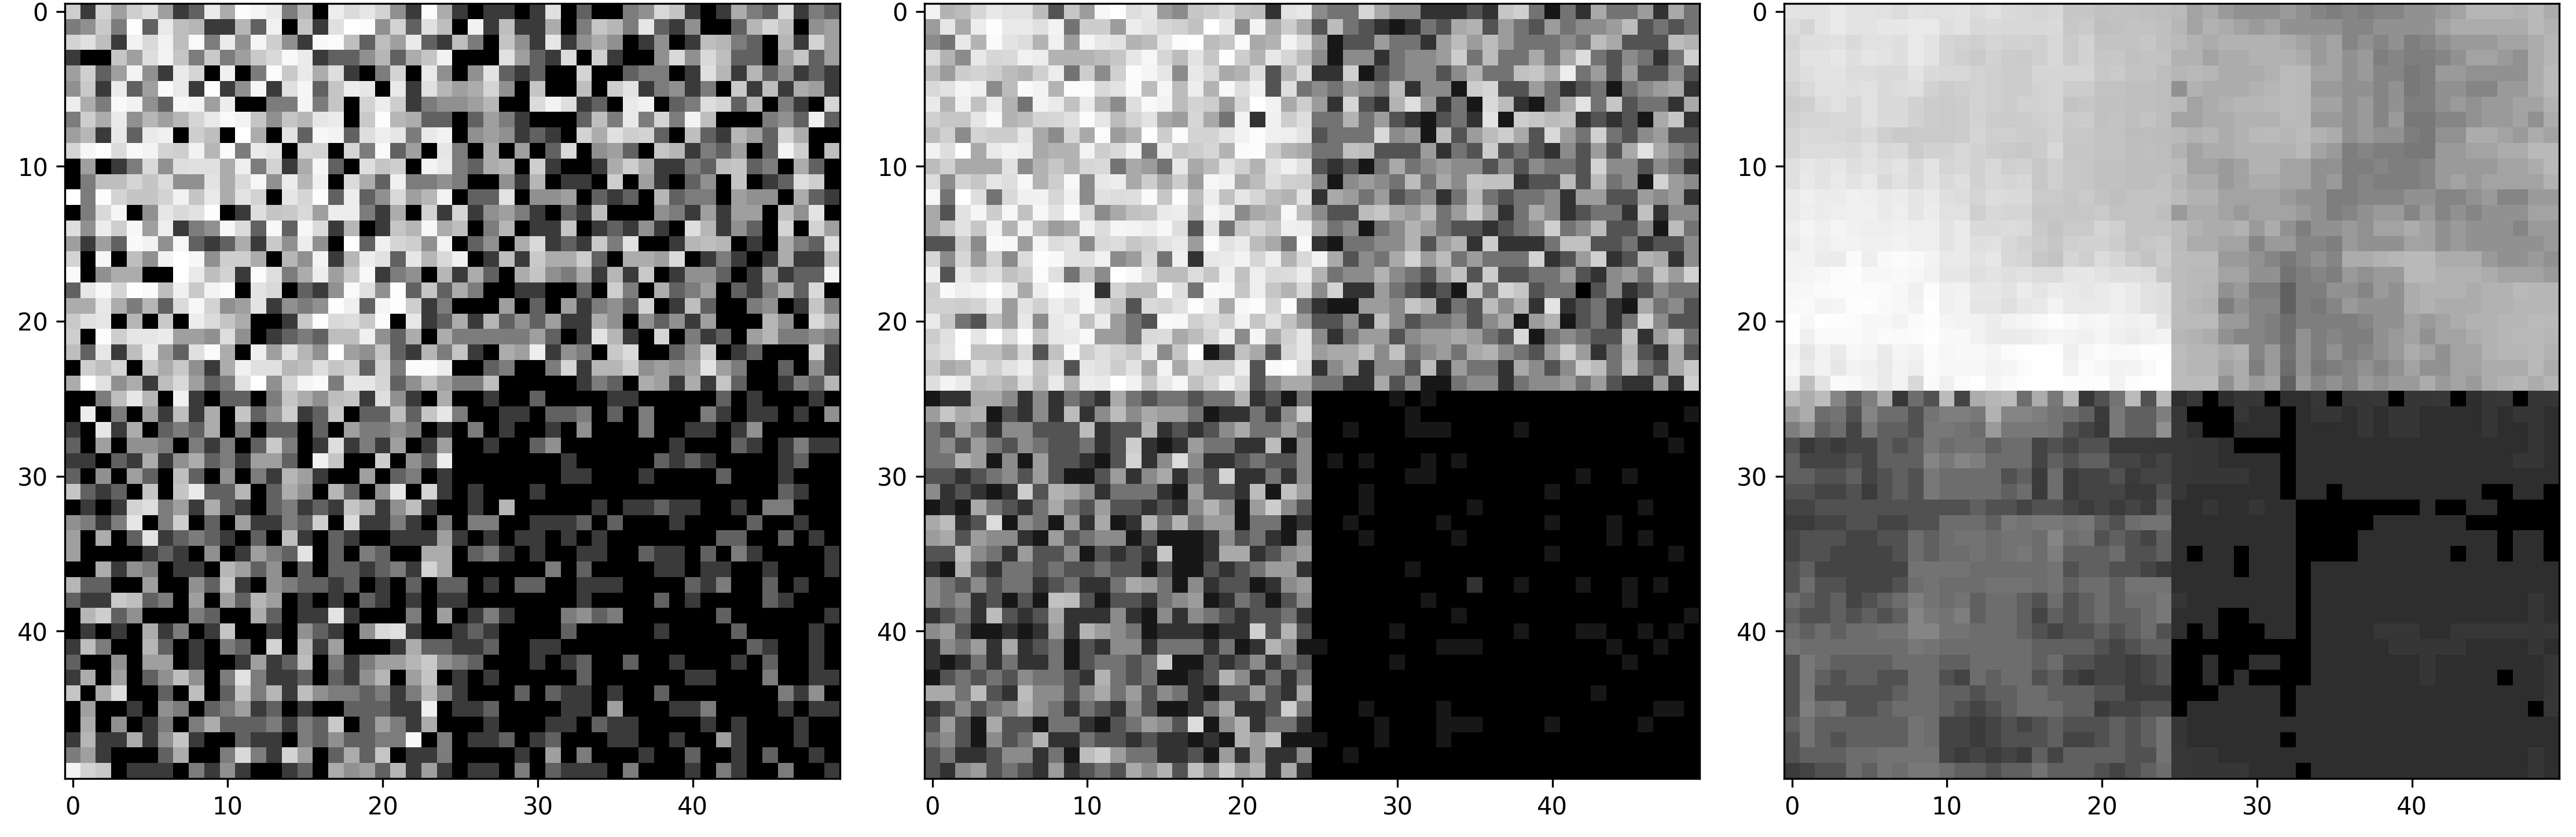
\includegraphics[width=0.9\textwidth]{Images/imtest_A15.png}
    \caption{Visual result of the A15 filter on a synthetic test image. From left to right: filtered output, original clean target, and noisy input. The model effectively removes noise but introduces artificial smoothness.}
    \label{fig:imtest_A15}
\end{figure}

\subsection{Performance on Real SAR Images}
To assess the generalization capabilities of our approach, the best model (A15) was applied to real SAR images. Figure \ref{fig:sar_munich_filtered} shows the result on a complex urban scene of Munich.

The filter successfully reduces a significant amount of the visible speckle, especially in smoother regions like parks or large rooftops. However, the model's limitations become apparent. Having been trained exclusively on simple, artificially generated quadrant images, the autoencoder did not learn the complex textures and structures inherent to real-world SAR data. As a result, it tends to over-smooth fine details and can sometimes create artifacts that do not correspond to the underlying scene. This highlights a key trade-off: while synthetic data allows for controlled training and evaluation, it may not equip the model with the robustness needed for the variability of real-world scenarios.

\begin{figure}[htbp]
    \centering
    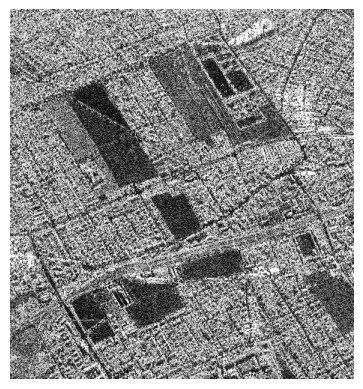
\includegraphics[width=0.7\textwidth]{Images/sar_munich.jpg}
    \caption{Application of the A15 filter to the original real SAR image of Munich (shown). On applying the filter, speckle is visibly reduced, particularly in homogeneous regions. However, as the model was trained on synthetic data, it tends to over-smooth complex textures and fine details present in the real scene.}
    \label{fig:sar_munich_filtered}
\end{figure}

\subsection{Statistical Evaluation and Comparative Analysis}

Finally, we performed a comparative analysis using the statistical figure of merit $\mathcal{M}$ described in the methods section, which combines mean preservation and residual structure analysis. We compared our best-performing autoencoders against the well-established Lee filter, a standard benchmark in speckle reduction. The results are summarized in Table \ref{tab:stat_results}.

\begin{table}[htbp]
\centering
\caption{Statistical figure of merit $\mathcal{M}$ for the top autoencoders compared to the Lee filter. A lower value indicates better overall performance.}
\label{tab:stat_results}
\begin{tabular}{|l|c|}
\hline
\textbf{Filter} & \textbf{Figure of Merit ($\mathcal{M}$)} \\
\hline
\textbf{Autoencoder A15} & \textbf{0.69} \\
Autoencoder A16 & 0.72 \\
Lee Filter (7x7) & 0.85 \\
\hline
\end{tabular}
\end{table}

The results show that our proposed autoencoder architectures, particularly A15, outperform the traditional Lee filter. They achieve a better balance of noise reduction (contributing to a higher ENL) and structure preservation, as captured by the lower $\mathcal{M}$ value. This demonstrates that, despite the limitations observed, the data-driven approach of a convolutional autoencoder can provide a superior despeckling performance compared to classic filtering techniques.
